% !TeX spellcheck = de_DE_frami
%%%%%%%%%%%%%%%%%%%%%%%%%%%%%%%%%%%%%%%%%%%%%%%%
% COPYRIGHT: (C) 2026 FAU FabLab and others
% CC-BY-SA 3.0
% Text in eigenen Worten, KEINE Passagen oder Abbildungen aus der
% Festool-Betriebsanleitung übernehmen (siehe README, Abschnitt Lizenz).
% Die Zeichnungen in zeichnungen/ sind selbst mit TikZ erstellt,
% Fotos nur mit freier Lizenz (siehe bilder/QUELLEN.md).
%%%%%%%%%%%%%%%%%%%%%%%%%%%%%%%%%%%%%%%%%%%%%%%%

\newcommand{\basedir}{fablab-document}
\documentclass{\basedir/fablab-document}

\usepackage{amssymb}
\usepackage{textcomp}
\usepackage{tabularx} % Tabellen mit bestimmtem Breitenverhältnis der Spalten
\usepackage{caption}
\usepackage{qrcode}
\usepackage{fablab-document/fablab-ba} % Betriebsanweisung
% =====================================================================
%  Gemeinsame Farben und Stile der Zeichnungen (TikZ, selbst erstellt)
%  In der Präambel einbinden: % =====================================================================
%  Gemeinsame Farben und Stile der Zeichnungen (TikZ, selbst erstellt)
%  In der Präambel einbinden: % =====================================================================
%  Gemeinsame Farben und Stile der Zeichnungen (TikZ, selbst erstellt)
%  In der Präambel einbinden: \input{zeichnungen/stil}
%  Lizenz wie das Dokument: CC BY-SA 3.0
% =====================================================================
\usetikzlibrary{calc,arrows.meta}

\definecolor{okgruen}{RGB}{46,160,67}
\definecolor{nokrot}{RGB}{207,34,46}
\definecolor{feld}{RGB}{244,246,248}
\definecolor{holz}{RGB}{226,196,150}
\definecolor{holzrand}{RGB}{150,110,60}
\definecolor{nut}{RGB}{186,150,100}
\definecolor{bediengruen}{RGB}{130,200,60}  % Grün der Bedienelemente

\tikzset{
  % Bauteile der Maschine
  gehaeuse/.style={fill=black!12, draw=black!75, line width=0.7pt, line join=round},
  griff/.style={fill=black!65, draw=black!85, line width=0.7pt, line join=round},
  metall/.style={fill=black!30, draw=black!75, line width=0.6pt, line join=round},
  werkstueck/.style={fill=holz, draw=holzrand, line width=0.6pt, line join=round},
  fraeser/.style={fill=black!55, draw=black!85, line width=0.5pt, line join=round},
  % Pfeile, Maße, Beschriftung
  vorschub/.style={-{Stealth[length=2.6mm, width=2.2mm]}, line width=1.3pt},
  drehung/.style={-{Stealth[length=1.8mm, width=1.6mm]}, line width=0.9pt},
  mass/.style={{Stealth[length=1.4mm]}-{Stealth[length=1.4mm]}, line width=0.4pt, black!80},
  hilfslinie/.style={line width=0.3pt, black!60},
  marke/.style={circle, draw=black, fill=white, line width=0.8pt,
    minimum size=4.4mm, inner sep=0pt, font=\scriptsize\bfseries},
  leitung/.style={line width=0.5pt, black!80},
  % Bewertung: \pic at (x,y) {ok}; bzw. {nok}
  ok/.pic={\fill[okgruen] (0,0) circle (3);
    \draw[white, line width=1.3pt, line cap=round, line join=round]
      (-1.4,0.1) -- (-0.4,-1.1) -- (1.5,1.2);},
  nok/.pic={\fill[nokrot] (0,0) circle (3);
    \draw[white, line width=1.3pt, line cap=round]
      (-1.1,-1.1) -- (1.1,1.1) (-1.1,1.1) -- (1.1,-1.1);},
}

% Feld mit hellem Hintergrund und Überschrift: \feld{x}{y}{Breite}{Höhe}{Titel}
\newcommand{\feld}[5]{%
  \fill[feld, rounded corners=2mm] (#1,#2) rectangle ++(#3,#4);
  \node[anchor=north west, font=\small\bfseries] at (#1+3,#2+#4-2) {#5};}

%  Lizenz wie das Dokument: CC BY-SA 3.0
% =====================================================================
\usetikzlibrary{calc,arrows.meta}

\definecolor{okgruen}{RGB}{46,160,67}
\definecolor{nokrot}{RGB}{207,34,46}
\definecolor{feld}{RGB}{244,246,248}
\definecolor{holz}{RGB}{226,196,150}
\definecolor{holzrand}{RGB}{150,110,60}
\definecolor{nut}{RGB}{186,150,100}
\definecolor{bediengruen}{RGB}{130,200,60}  % Grün der Bedienelemente

\tikzset{
  % Bauteile der Maschine
  gehaeuse/.style={fill=black!12, draw=black!75, line width=0.7pt, line join=round},
  griff/.style={fill=black!65, draw=black!85, line width=0.7pt, line join=round},
  metall/.style={fill=black!30, draw=black!75, line width=0.6pt, line join=round},
  werkstueck/.style={fill=holz, draw=holzrand, line width=0.6pt, line join=round},
  fraeser/.style={fill=black!55, draw=black!85, line width=0.5pt, line join=round},
  % Pfeile, Maße, Beschriftung
  vorschub/.style={-{Stealth[length=2.6mm, width=2.2mm]}, line width=1.3pt},
  drehung/.style={-{Stealth[length=1.8mm, width=1.6mm]}, line width=0.9pt},
  mass/.style={{Stealth[length=1.4mm]}-{Stealth[length=1.4mm]}, line width=0.4pt, black!80},
  hilfslinie/.style={line width=0.3pt, black!60},
  marke/.style={circle, draw=black, fill=white, line width=0.8pt,
    minimum size=4.4mm, inner sep=0pt, font=\scriptsize\bfseries},
  leitung/.style={line width=0.5pt, black!80},
  % Bewertung: \pic at (x,y) {ok}; bzw. {nok}
  ok/.pic={\fill[okgruen] (0,0) circle (3);
    \draw[white, line width=1.3pt, line cap=round, line join=round]
      (-1.4,0.1) -- (-0.4,-1.1) -- (1.5,1.2);},
  nok/.pic={\fill[nokrot] (0,0) circle (3);
    \draw[white, line width=1.3pt, line cap=round]
      (-1.1,-1.1) -- (1.1,1.1) (-1.1,1.1) -- (1.1,-1.1);},
}

% Feld mit hellem Hintergrund und Überschrift: \feld{x}{y}{Breite}{Höhe}{Titel}
\newcommand{\feld}[5]{%
  \fill[feld, rounded corners=2mm] (#1,#2) rectangle ++(#3,#4);
  \node[anchor=north west, font=\small\bfseries] at (#1+3,#2+#4-2) {#5};}

%  Lizenz wie das Dokument: CC BY-SA 3.0
% =====================================================================
\usetikzlibrary{calc,arrows.meta}

\definecolor{okgruen}{RGB}{46,160,67}
\definecolor{nokrot}{RGB}{207,34,46}
\definecolor{feld}{RGB}{244,246,248}
\definecolor{holz}{RGB}{226,196,150}
\definecolor{holzrand}{RGB}{150,110,60}
\definecolor{nut}{RGB}{186,150,100}
\definecolor{bediengruen}{RGB}{130,200,60}  % Grün der Bedienelemente

\tikzset{
  % Bauteile der Maschine
  gehaeuse/.style={fill=black!12, draw=black!75, line width=0.7pt, line join=round},
  griff/.style={fill=black!65, draw=black!85, line width=0.7pt, line join=round},
  metall/.style={fill=black!30, draw=black!75, line width=0.6pt, line join=round},
  werkstueck/.style={fill=holz, draw=holzrand, line width=0.6pt, line join=round},
  fraeser/.style={fill=black!55, draw=black!85, line width=0.5pt, line join=round},
  % Pfeile, Maße, Beschriftung
  vorschub/.style={-{Stealth[length=2.6mm, width=2.2mm]}, line width=1.3pt},
  drehung/.style={-{Stealth[length=1.8mm, width=1.6mm]}, line width=0.9pt},
  mass/.style={{Stealth[length=1.4mm]}-{Stealth[length=1.4mm]}, line width=0.4pt, black!80},
  hilfslinie/.style={line width=0.3pt, black!60},
  marke/.style={circle, draw=black, fill=white, line width=0.8pt,
    minimum size=4.4mm, inner sep=0pt, font=\scriptsize\bfseries},
  leitung/.style={line width=0.5pt, black!80},
  % Bewertung: \pic at (x,y) {ok}; bzw. {nok}
  ok/.pic={\fill[okgruen] (0,0) circle (3);
    \draw[white, line width=1.3pt, line cap=round, line join=round]
      (-1.4,0.1) -- (-0.4,-1.1) -- (1.5,1.2);},
  nok/.pic={\fill[nokrot] (0,0) circle (3);
    \draw[white, line width=1.3pt, line cap=round]
      (-1.1,-1.1) -- (1.1,1.1) (-1.1,1.1) -- (1.1,-1.1);},
}

% Feld mit hellem Hintergrund und Überschrift: \feld{x}{y}{Breite}{Höhe}{Titel}
\newcommand{\feld}[5]{%
  \fill[feld, rounded corners=2mm] (#1,#2) rectangle ++(#3,#4);
  \node[anchor=north west, font=\small\bfseries] at (#1+3,#2+#4-2) {#5};}
 % Farben und Stile der Zeichnungen
% Farbe mit Farbfeld, Wort in etwas dunklerer Farbe (lesbar), z.B. \farbe{bediengruen}{grün}
\newcommand{\farbe}[2]{{\colorlet{farbefeld}{#1}\tikz[baseline=-0.6ex]\draw[fill=farbefeld, draw=black!60] (0,-1.1mm) rectangle (2.2mm,1.1mm);~\textcolor{farbefeld!70!black}{#2}}}

% Nummer eines Bedienelements wie in der Übersicht, z.B. \teil{3}
\newcommand{\teil}[1]{\tikz[baseline=(n.base)]\node[marke, minimum size=3.8mm, font=\tiny\bfseries](n){#1};}

\date{\today}
% Versionsnummer: version.tex wird von make erzeugt,
% ohne git steht stattdessen "Entwurf" mit Datum in der Fußzeile.
\InputIfFileExists{version}{}{\newcommand{\Version}{Entwurf \today}}
\fancyfoot[R]{Version \Version}
\author{kontakt@fablab.fau.de}
\title{Einweisung Dübelfräse}

\begin{document}

	\maketitle
	\begin{center}
		Für die Dübelfräse \textbf{Festool DOMINO DF 500 RQ-Plus}\\[1mm]
		{\small Version \Version}
	\end{center}

	\textbf{Nur eingewiesene Benutzer dürfen die Dübelfräse selbstständig benutzen.}
	Wenn du noch nicht eingewiesen bist, frage einen Betreuer. Nach der Einweisung und Unterschrift darfst du die Dübelfräse selbstständig verwenden.

	\section{Regeln und Sicherheit}

	\begin{itemize}
		\item Das Werkstück ist immer \textbf{fest gespannt} oder liegt bei großen Platten sicher auf. Kleine Teile nie mit der Hand halten.
		\item Die Fräse wird immer mit \textbf{beiden Händen} geführt: eine Hand am Motorgehäuse, eine am Griff des Fräsanschlags.
		\item Hände nie vor die Stirnseite der Fräse halten: Dort tritt der Fräser beim Eintauchen heraus.
		\item Erst ansetzen, dann einschalten, dann eintauchen. Nach dem Fräsen ausschalten und warten, bis der Fräser steht.
		\item Immer mit angeschlossener Absaugung fräsen.
		\item Gehörschutz und Schutzbrille tragen, bei viel Staub (Hartholz) zusätzlich Staubmaske. Beim Fräsen \textbf{keine Handschuhe}.
		\item Fräser nur bei \textbf{gezogenem Netzstecker} wechseln.
		\item Nur Holz und Holzwerkstoffe fräsen.
		\item Netzkabel und Saugschlauch aus dem Arbeitsbereich fernhalten.
		\item Im Arbeitsbereich dürfen sich keine Unbeteiligten aufhalten.
		\item Schäden an der Fräse sofort melden: \texttt{fablab-aktive@fablab.fau.de}.
	\end{itemize}

	\BAfalls{betriebsanweisung/ba_duebelfraese}{Zusätzlich gilt die \textbf{Betriebsanweisung} auf der nächsten Seite (Abschnitt~\ref{sec:betriebsanweisung}). Sie hängt bei der Dübelfräse aus und ist Bestandteil dieser Einweisung.}

	\newpage

	% Betriebsanweisung als ganze Seite im Format des Aushangs
	\BAseite[sec:betriebsanweisung]{betriebsanweisung/ba_duebelfraese}

	\renewcommand{\contentsname}{Inhaltsverzeichnis / Arbeitsablauf}
	\setcounter{tocdepth}{2}
	\tableofcontents
	\newpage

	\section{Die Dübelfräse und ihre Anleitung}

	\begin{center}
		\begin{tabular}{r|l}
			Hersteller & Festool \\
			Produktname & Dübelfräse DOMINO DF 500 RQ-Plus \\
			Leistung & $420\,\mathrm{Watt}$ \\
			Drehzahl & $25.500\,\mathrm{min}^{-1}$ \\
			Fräserdurchmesser & $4$, $5$, $6$, $8$ und $10\,\mathrm{mm}$ \\
			Frästiefe & $12$, $15$, $20$, $25$ oder $28\,\mathrm{mm}$ \\
			Fräshöhe & $5 - 30\,\mathrm{mm}$ \\
			Fräswinkel & $0 - 90$\textdegree \\
			Dübel & $4 \times 20$ bis $10 \times 50\,\mathrm{mm}$ \\
			Absauganschluss & $27\,\mathrm{mm}$ \\
		\end{tabular}
	\end{center}

	\subsection{Bedienelemente}
	\label{sec:bedienelemente}

	Die Fotos zeigen die Dübelfräse des FabLabs. Die Nummern werden in der ganzen Einweisung verwendet.

	\begin{center}
		% =====================================================================
%  Eigene Fotos der Dübelfräse im FabLab mit nummerierten Bedienelementen.
%  Koordinaten relativ zum jeweiligen Foto: (0,0) unten links, (1,1) oben rechts.
%  Nummern wie in der Tabelle in einweisung_Duebelfraese.tex
% =====================================================================
% \fotonr{Nummer}{Position der Nummer}{Bauteil}, nur innerhalb eines Foto-Scopes
\newcommand{\fotonr}[3]{%
  \draw[white, line width=2pt, line cap=round] (#2) -- (#3);
  \draw[black, line width=0.8pt] (#2) -- (#3);
  \fill[black] (#3) circle[radius=0.7mm];
  \node[marke, minimum size=5.5mm, font=\small\bfseries, line width=1pt] at (#2) {#1};}
\newcommand{\fototitel}[1]{\node[anchor=north west, fill=white, fill opacity=0.85,
  text opacity=1, font=\small\bfseries, inner sep=1.2mm] at (0,1) {#1};}

\begin{tikzpicture}
  \node[anchor=south west, inner sep=0pt] (a) at (0,0)
    {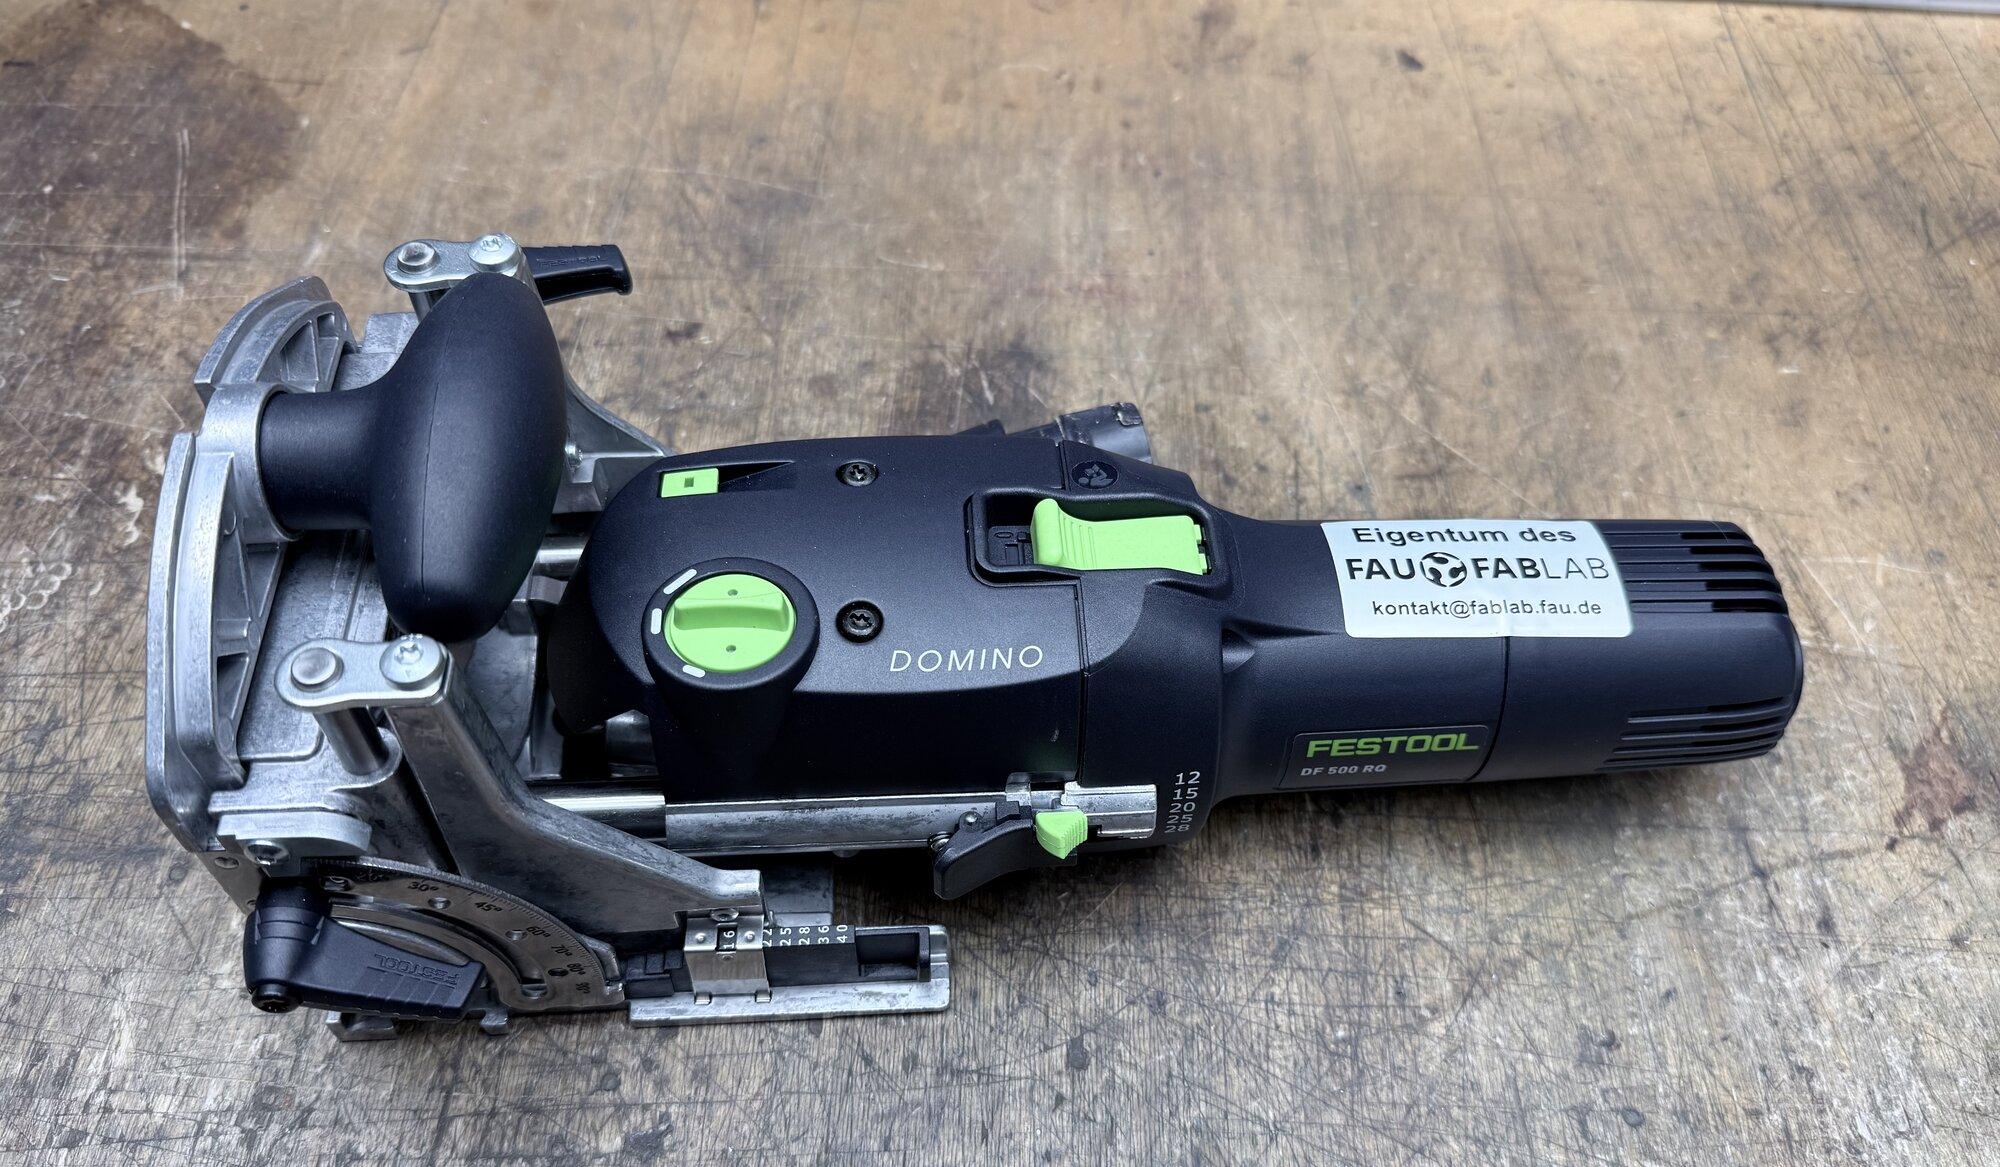
\includegraphics[width=\textwidth]{bilder/domino-oben.jpg}};
  \begin{scope}[x={(a.south east)}, y={(a.north west)}]
    \fotonr{1}{0.60,0.82}{0.557,0.543}
    \fotonr{2}{0.93,0.80}{0.88,0.55}
    \fotonr{3}{0.12,0.88}{0.219,0.613}
    \fotonr{4}{0.38,0.85}{0.365,0.468}
    \fotonr{5}{0.56,0.10}{0.529,0.292}
    \fotonr{6}{0.07,0.12}{0.183,0.253}
  \end{scope}
\end{tikzpicture}

\vspace{2mm}
\begin{tikzpicture}
  \node[anchor=south west, inner sep=0pt] (b) at (0,0)
    {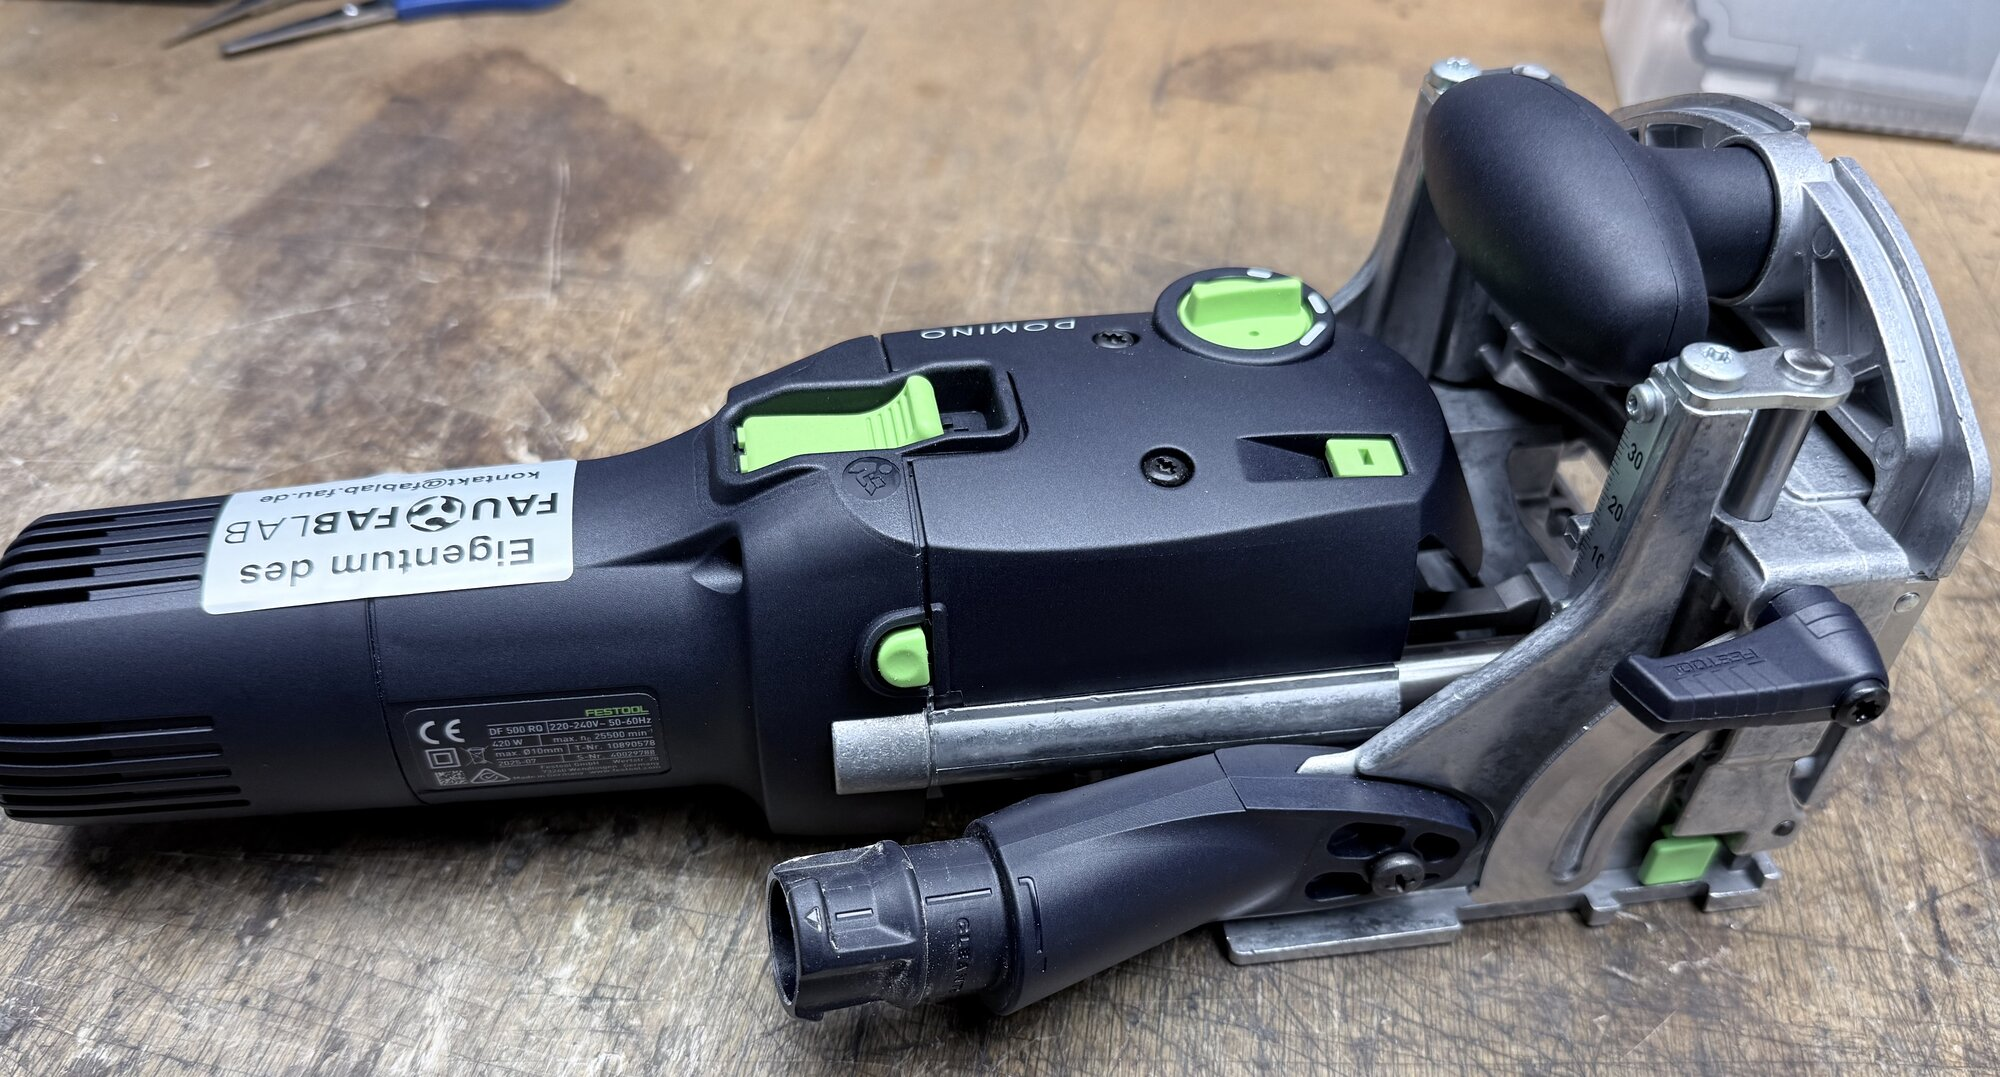
\includegraphics[width=0.6\textwidth]{bilder/domino-seite.jpg}};
  \node[anchor=south west, inner sep=0pt] (c) at ([xshift=0.02\textwidth]b.south east)
    {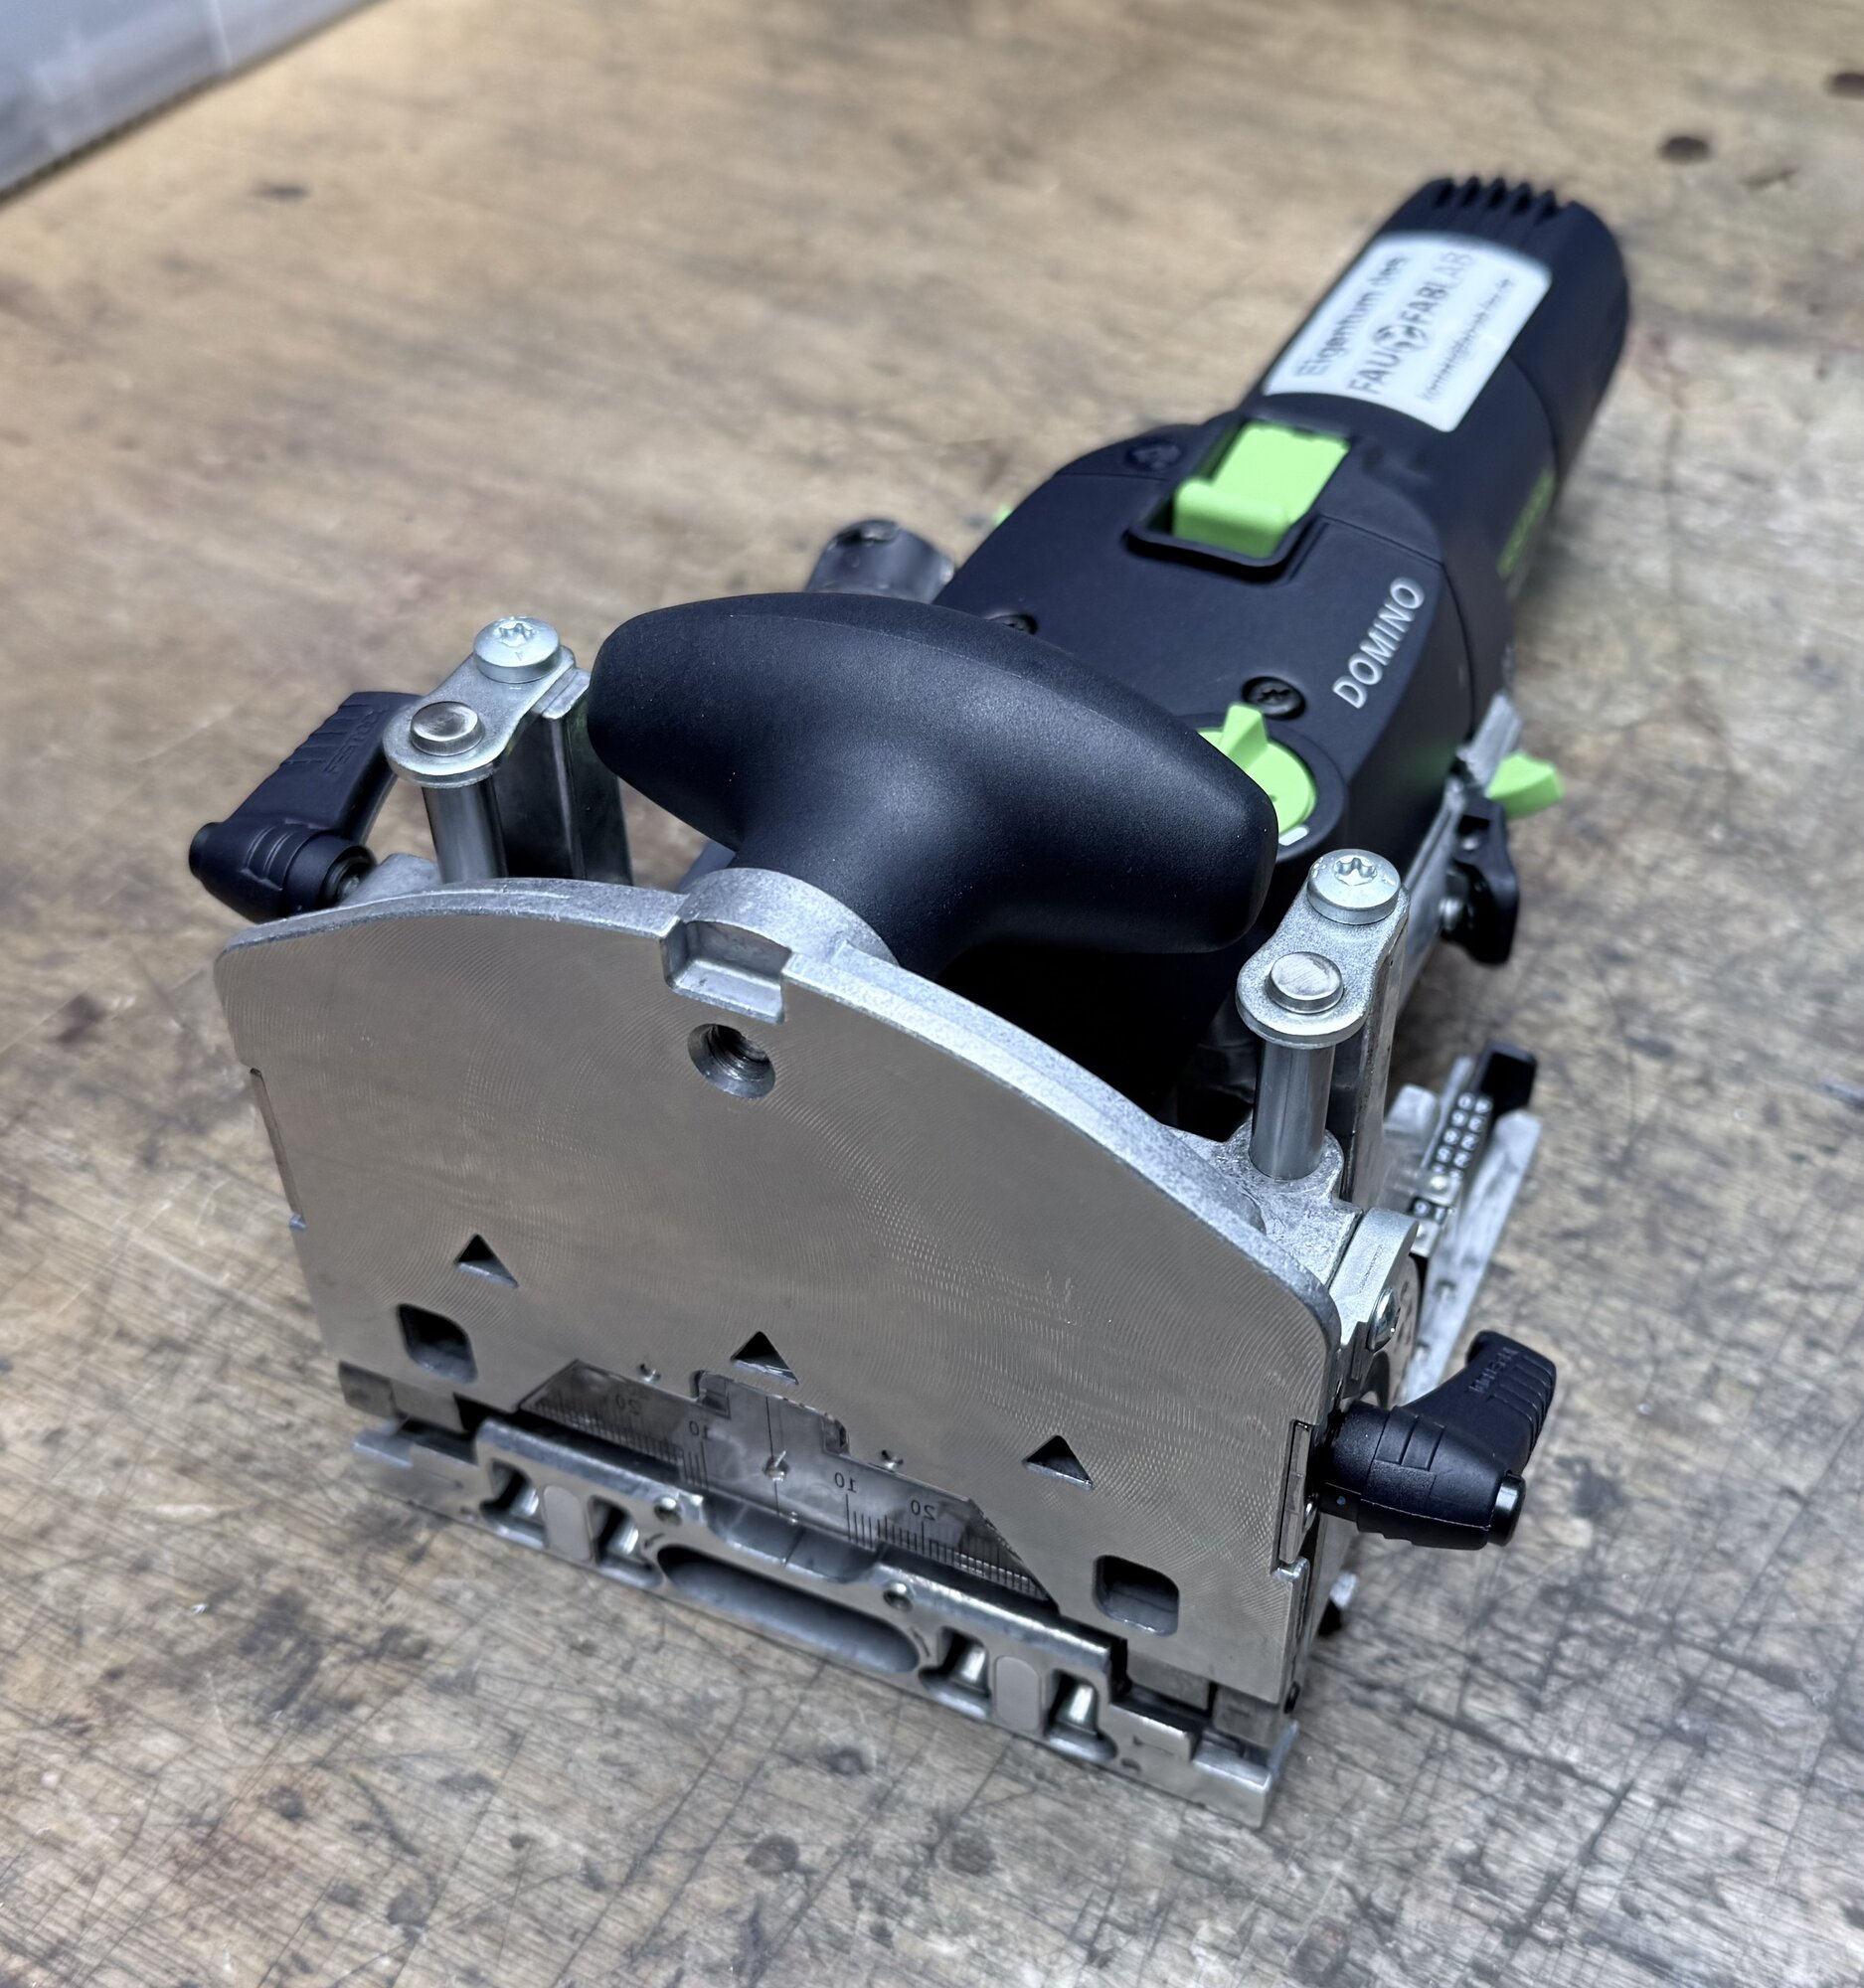
\includegraphics[height=0.3229\textwidth]{bilder/domino-vorn.jpg}};
  \begin{scope}[x={(b.south east)}, y={(b.north west)}]
    \fotonr{7}{0.70,0.88}{0.802,0.525}
    \fotonr{8}{0.95,0.18}{0.858,0.389}
    \fotonr{9}{0.20,0.12}{0.414,0.139}
  \end{scope}
  \begin{scope}[shift={(c.south west)}, x={($(c.south east)-(c.south west)$)}, y={($(c.north west)-(c.south west)$)}]
    \fotonr{10}{0.14,0.14}{0.406,0.323}
  \end{scope}
\end{tikzpicture}

	\end{center}

	\begin{center}
		\small
		\renewcommand{\arraystretch}{1.25}
		\renewcommand{\tabularxcolumn}[1]{m{#1}}
		\begin{tabularx}{\textwidth}{|c|m{42mm}|X|}
			\hline
			& \textbf{Bedienelement} & \textbf{Bedienung} \\ \hline
			\teil{1} & Ein-/Ausschalter (\farbe{bediengruen}{grün}, oben) & Schiebeschalter, rastet ein: Die Fräse läuft, bis du ihn wieder zurückschiebst. \\ \hline
			\teil{2} & Motorgehäuse & Eine Hand. Beim Eintauchen schiebst du den Motor nach vorn, eine Feder drückt ihn danach zurück. \\ \hline
			\teil{3} & Griff am Fräsanschlag & Zweite Hand. Drückt die Fräse an das Werkstück. \\ \hline
			\teil{4} & Drehknopf Langlochbreite (\farbe{bediengruen}{grün}) & Drei Stellungen: eng, mittel, weit (Abschnitt~\ref{sec:prinzip}). \\ \hline
			\teil{5} & Tiefenanschlag (\farbe{bediengruen}{grüner} Schieber, Skala 12--28) & Frästiefe passend zum Dübel einrasten (Abschnitt~\ref{sec:duebel}). \\ \hline
			\teil{6} & Winkelskala & Winkel des Fräsanschlags von 0\textdegree{} bis 90\textdegree{} ablesen. \\ \hline
			\teil{7} & Höhenskala & Höhe des Langlochs ablesen (Abschnitt~\ref{sec:hoehe}). \\ \hline
			\teil{8} & Klemmhebel & Lösen, Höhe einstellen, wieder festklemmen. \\ \hline
			\teil{9} & Absauganschluss & Saugschlauch aufstecken. Nie ohne Absaugung fräsen. \\ \hline
			\teil{10} & Stirnseite mit Markierungen & Liegt flach an der Werkstückkante an. Die Dreiecke zeigen die Lage des Fräsers, die mittlere Markierung auf den Bleistiftstrich ausrichten. \\ \hline
		\end{tabularx}
	\end{center}

	So liegt die Fräse beim Fräsen eines Langlochs in die Stirnseite eines Werkstücks am Werkstück an (schematisch):

	\begin{center}
		% =====================================================================
%  Dübelfräse beim Fräsen eines Langlochs in die Stirnseite eines
%  Werkstücks: schematisch von der Seite, nicht maßstäblich.
%  Selbst gezeichnet. Nummern wie in der Legende in einweisung_Duebelfraese.tex
% =====================================================================
\begin{tikzpicture}[x=0.85mm, y=0.85mm, font=\scriptsize]
  % Werkbank und Werkstück mit Langloch
  \fill[black!8] (-52,-4) rectangle (128,0);
  \draw[black!40, line width=0.5pt] (-52,0) -- (128,0);
  \draw[werkstueck] (-50,0) rectangle (0,19);
  \fill[nut] (-16,6) rectangle (0,13);
  \node at (-33,9.5) {Werkstück};

  % Fräser (eingetaucht) mit Schaft
  \draw[fraeser, fill=black!35] (-3,8.3) rectangle (6,10.7);
  \draw[fraeser] (-15,7) rectangle (-3,12);
  \draw[white, line width=0.5pt] (-13,7) -- (-10,12) (-8,7) -- (-5,12);

  % Absauganschluss und Netzkabel (hinten)
  \draw[gehaeuse, fill=black!30] (104,1) rectangle (120,8);
  \draw[gehaeuse, fill=black!45] (118,0) rectangle (121,9);
  \draw[black!85, line width=1.6pt] (110,20) to[out=0,in=180] (126,26);

  % Motorgehäuse mit Ein-/Ausschalter oben
  \draw[gehaeuse, rounded corners=4] (22,4) rectangle (112,30);
  \foreach \x in {88,92,...,104}
    \draw[black!50, line width=0.8pt, line cap=round] (\x,10) -- (\x,24);
  \draw[fill=bediengruen, draw=black!80, line width=0.5pt, rounded corners=1] (58,30) rectangle (72,33);

  % Vorderteil (Fräskorb) mit Grundplatte
  \draw[gehaeuse, fill=black!20, rounded corners=1.5] (0,0) rectangle (24,27);
  \draw[metall, fill=black!40] (0,0) rectangle (40,3);
  \fill[black!70] (0,6) rectangle (1.5,13);

  % Fräsanschlag auf dem Werkstück, Griff obendrauf
  \draw[metall, fill=black!30] (-16,19) rectangle (10,23);
  \draw[metall, fill=black!30] (4,19) rectangle (10,32);
  \draw[griff, rounded corners=3] (2,32) rectangle (26,38);
  % Anschlagbolzen
  \draw[fill=black!70, draw=black!90] (-1.5,23) rectangle (0,27);

  % Eintauchrichtung
  \draw[vorschub] (108,37) -- (84,37);
  \node[anchor=south] at (96,38.5) {Eintauchen};

  % Nummern
  \newcommand{\nr}[3]{\draw[leitung] (#2) -- (#3); \node[marke] at (#2) {#1};}
  \nr{1}{65,46}{65,33}
  \nr{2}{80,-10}{80,4}
  \nr{3}{14,46}{14,38}
  \nr{4}{-24,30}{-12,23}
  \nr{5}{-22,-10}{-12,7}
  \nr{6}{12,-10}{12,1.5}
  \nr{7}{-8,34}{-1,27}
  \nr{8}{112,-10}{112,4.5}
\end{tikzpicture}

	\end{center}

	\subsection{Anleitung und bestimmungsgemäße Verwendung}

	Diese Einweisung fasst die Regeln des FabLabs zusammen und erklärt die Bedienung in eigenen Worten. Sie ersetzt nicht die Betriebsanleitung des Herstellers: Die \textbf{Originalbetriebsanleitung} liegt der Maschine bei. Was hier nicht beschrieben ist (Zubehör, weitere Anschläge, Ersatzteile), steht dort.

	\begin{center}
		\begin{tabular}{cc}
			\qrcode[height=2.2cm]{https://www.festool.de/bedienungsanleitungen} &
			\qrcode[height=2.2cm]{https://www.festool.de/produkte/domino-verbindungssystem/duebelfraesen} \\[1mm]
			\href{https://www.festool.de/bedienungsanleitungen}{Bedienungsanleitungen} &
			\href{https://www.festool.de/produkte/domino-verbindungssystem/duebelfraesen}{Dübelfräsen bei Festool}
		\end{tabular}
	\end{center}

	Die Dübelfräse fräst Langlöcher für DOMINO-Dübel in Holz und Holzwerkstoffe, zum Beispiel für Eck-, T- und Flächenverbindungen von Platten, Rahmen und Gestellen. Sie wird von Hand geführt.

	\section{So funktioniert die Dübelverbindung}

	\subsection{Langloch und Dübel}
	\label{sec:prinzip}
	Der Fräser dreht sich und pendelt dabei seitlich hin und her. So entsteht kein rundes Loch wie beim Bohren, sondern ein \textbf{Langloch}. In beide Teile wird an der gleichen Stelle ein Langloch gefräst, der flache DOMINO-Dübel wird eingeleimt und verbindet die Teile.

	\begin{center}
		% =====================================================================
%  Prinzip der Dübelfräse: Langloch, Langlochbreiten, Reihenfolge eng/weit,
%  fertige Verbindung. Ansicht auf die Stirnseite bzw. Schnitt. Selbst gezeichnet.
% =====================================================================
\begin{tikzpicture}[x=1mm, y=1mm, font=\scriptsize,
    langloch/.style={fill=black!70, rounded corners=2.4},
    duebel/.style={draw=holz, dashed, line width=0.7pt, rounded corners=2.4}]

  % ---------------- 1 Langloch -------------------------------------
  \feld{0}{50}{82}{46}{1\quad Fräser dreht und pendelt}
  \begin{scope}[shift={(0,50)}]
    \draw[werkstueck] (8,10) rectangle (74,31);
    \fill[langloch] (29,18) rectangle (53,23.5);
    \fill[black!35] (41,20.75) circle (2.6);
    \draw[drehung, okgruen] (41,20.75) ++(160:4.2) arc[start angle=160, end angle=20, radius=4.2];
    \draw[mass, line width=0.8pt, okgruen] (30,27.5) -- (52,27.5);
    \node[anchor=west] at (54,27.5) {pendeln};
    \node[align=center] at (41,5) {Stirnseite des Werkstücks: es entsteht ein Langloch};
  \end{scope}

  % ---------------- 2 Langlochbreiten ------------------------------
  \feld{88}{50}{82}{46}{2\quad Drei Langlochbreiten}
  \begin{scope}[shift={(88,50)}]
    \draw[werkstueck] (6,13) rectangle (76,31);
    \fill[langloch] (9,19.5) rectangle (23,24.5);
    \fill[langloch] (30,19.5) rectangle (47,24.5);
    \fill[langloch] (54,19.5) rectangle (74,24.5);
    \foreach \x in {9.3,31.8,57.3}
      \draw[duebel] (\x,19.8) rectangle ++(13.4,4.4);
    \node at (16,9) {eng};
    \node at (38.5,9) {mittel};
    \node at (64,9) {weit};
    \node[align=center] at (41,4) {gestrichelt: Dübel};
  \end{scope}

  % ---------------- 3 Reihenfolge ----------------------------------
  \feld{0}{0}{82}{46}{3\quad Erst eng, dann weit}
  \begin{scope}[shift={(0,0)}]
    \draw[werkstueck] (4,16) rectangle (78,30);
    \fill[langloch] (10,20.5) rectangle (24,25.5);
    \fill[langloch] (34,20.5) rectangle (52,25.5);
    \fill[langloch] (57,20.5) rectangle (75,25.5);
    \node at (17,12) {eng};
    \node at (43,12) {weit};
    \node at (66,12) {weit};
    \node[align=center] at (41,5) {das erste Langloch legt die Lage fest};
  \end{scope}

  % ---------------- 4 Verbindung -----------------------------------
  \feld{88}{0}{82}{46}{4\quad Fertige Verbindung (Schnitt)}
  \begin{scope}[shift={(88,0)}]
    \draw[werkstueck] (6,14) rectangle (40,30);
    \draw[werkstueck] (42,14) rectangle (76,30);
    \fill[nut] (27,19.5) rectangle (40,24.5) (42,19.5) rectangle (55,24.5);
    \draw[fill=holz!70!white, draw=holzrand, line width=0.5pt, rounded corners=1.2] (28.5,19.8) rectangle (53.5,24.2);
    \draw[holzrand, line width=0.3pt] \foreach \x in {31,34,...,52} {(\x,20) -- (\x+1.5,24)};
    \draw[mass] (27,33) -- (40,33);
    \draw[hilfslinie] (27,24.5) -- (27,34) (40,30) -- (40,34);
    \node[anchor=south] at (33.5,33.5) {Frästiefe};
    \node[align=center] at (41,6) {Frästiefe je Teil mindestens\\halbe Dübellänge};
  \end{scope}
\end{tikzpicture}

	\end{center}

	\begin{itemize}
		\item Die Langlochbreite lässt sich in drei Stufen wählen: \textbf{eng} (so breit wie der Dübel), \textbf{mittel} und \textbf{weit} (mit seitlichem Spiel).
		\item Pro Verbindung wird das erste Langloch in jedem Teil \textbf{eng} gefräst. Es legt die Lage der Teile zueinander fest. Die weiteren Langlöcher werden weit gefräst. Das Spiel gleicht kleine Ungenauigkeiten beim Anzeichnen aus, die Teile lassen sich trotzdem bündig zusammenstecken.
	\end{itemize}

	\begin{center}
		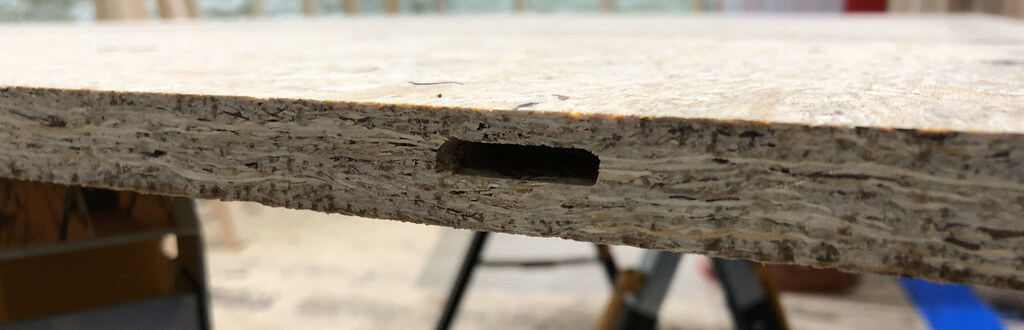
\includegraphics[width=0.8\textwidth]{bilder/domino-langloch.jpg}\\[1mm]
		{\footnotesize Langloch in der Kante einer Spanplatte.
		Foto: Pete Brown, \href{https://www.flickr.com/photos/34452246@N02/39827901651}{Flickr}, Lizenz \href{https://creativecommons.org/licenses/by/2.0/}{CC BY 2.0}, Ausschnitt.}
	\end{center}

	\subsection{Dübel, Fräser und Frästiefe}
	\label{sec:duebel}
	Fräser und Frästiefe richten sich nach dem Dübel. Die Frästiefe je Teil muss mindestens die halbe Dübellänge betragen, sonst stößt der Dübel an und die Fuge bleibt offen. Gewählt wird die nächste passende Stufe des Tiefenanschlags.

	\begin{center}
		\small
		\renewcommand{\arraystretch}{1.3}
		\begin{tabular}{|l|c|c|}
			\hline
			\textbf{Dübel (Dicke $\times$ Länge)} & \textbf{Fräser} & \textbf{Frästiefe je Teil} \\ \hline
			$4 \times 20$\,mm & 4\,mm & 12\,mm \\ \hline
			$5 \times 30$\,mm & 5\,mm & 15\,mm \\ \hline
			$6 \times 40$\,mm & 6\,mm & 20\,mm \\ \hline
			$8 \times 40$\,mm & 8\,mm & 20\,mm \\ \hline
			$8 \times 50$\,mm & 8\,mm & 25\,mm \\ \hline
			$10 \times 50$\,mm & 10\,mm & 25\,mm \\ \hline
		\end{tabular}
	\end{center}

	Faustregel: Der Dübel ist etwa ein Drittel so dick wie das Material, also z.\,B.\ 6\,mm-Dübel bei 19\,mm Plattenstärke.

	\section{Vorbereitung}

	\subsection{Checkliste vor dem Fräsen}
	Vor \textbf{jedem} Einsatz durchgehen:
	\begin{itemize}
		\item Fräse, Netzkabel und Saugschlauch unbeschädigt?
		\item Richtiger Fräser für den Dübel eingesetzt, scharf und unbeschädigt?
		\item Frästiefe, Langlochbreite, Höhe und Winkel eingestellt und alle Klemmungen fest?
		\item Schutzausrüstung angelegt (siehe unten)?
		\item Absaugung angeschlossen, Sauger auf \enquote{AUTO}?
		\item Werkstück fest gespannt, Anrisse auf beiden Teilen?
		\item Ein-/Ausschalter~\teil{1} in Stellung Aus, bevor der Netzstecker eingesteckt wird?
		\item Arbeitsbereich frei, keine Unbeteiligten in der Nähe?
	\end{itemize}

	\subsection{Schutzausrüstung}
	\begin{itemize}
		\item Gehörschutz: immer.
		\item Schutzbrille: immer, Späne können seitlich herausfliegen.
		\item Staubmaske bei stauberzeugenden Arbeiten, insbesondere bei Hartholz.
		\item Beim Fräsen \textbf{keine Handschuhe} tragen: Der rotierende Fräser kann sie erfassen und die Hand mitziehen. Schutzhandschuhe nur, wenn die Fräse steht: beim Fräserwechsel mit gezogenem Netzstecker und beim Tragen von rauem Material.
		\item Eng anliegende Kleidung ohne Fransen, Schals oder Kordeln, keinen Schmuck. Lange Haare zusammenbinden.
	\end{itemize}

	\subsection{Material}
	\begin{itemize}
		\item Zugelassen: Massivholz und Holzwerkstoffe wie Spanplatte, MDF und Sperrholz.
		\item Nicht zugelassen: Metall, Kunststoff, Stein und Material mit Nägeln, Schrauben oder Klammern im Fräsbereich.
		\item Hartholzstaub ist gesundheitsschädlich. Bei Hartholz nur mit dem Sauger der Staubklasse M (oder besser) arbeiten.
	\end{itemize}

	\subsection{Absaugung}
	Immer mit dem Festool-Sauger fräsen. Den Netzstecker der Fräse in die Steckdose am Sauger stecken und den Sauger auf \enquote{AUTO} stellen: Er startet dann mit der Fräse und läuft nach dem Ausschalten kurz nach. Lässt die Absaugung nach, die Arbeit unterbrechen, den Netzstecker ziehen und Absauganschluss~\teil{9} und Schlauch auf Verstopfung prüfen.

	\subsection{Werkstück spannen und anzeichnen}
	\begin{itemize}
		\item Werkstücke mit geeigneten Spannmitteln fest spannen, z.\,B. mit Zwingen auf der Werkbank oder mit den Spannelementen am Multifunktionstisch (MFT). Die Spannmittel dürfen Fräse und Fräsanschlag nicht behindern.
		\item Beide Teile so hinlegen, wie sie später zusammengehören, und mit einem Bleistiftstrich quer über die Fuge die Lage jedes Dübels auf beiden Teilen anzeichnen.
		\item Die Sichtseiten markieren. Alle Langlöcher werden mit dem Fräsanschlag auf der Sichtseite gefräst (Abschnitt~\ref{sec:hoehe}).
	\end{itemize}

	\section{Einstellungen}

	\subsection{Fräser}
	Der Fräser muss zum Dübel passen (Tabelle in Abschnitt~\ref{sec:duebel}). Ist der falsche Fräser eingesetzt, einen Betreuer fragen. Der Wechsel erfolgt nur bei gezogenem Netzstecker (Abschnitt~\ref{sec:fraeserwechsel}).

	\subsection{Frästiefe}
	Der Tiefenanschlag~\teil{5} hat fünf Raststufen: 12, 15, 20, 25 und 28\,mm. Die Stufe passend zum Dübel einstellen (Tabelle in Abschnitt~\ref{sec:duebel}). In der Regel wird bei beiden Teilen einer Verbindung dieselbe Frästiefe eingestellt.

	\subsection{Langlochbreite}
	Am Drehknopf~\teil{4} zwischen \textbf{eng}, \textbf{mittel} und \textbf{weit} wählen. Das erste Langloch jedes Teils eng fräsen, danach auf weit umstellen (Abschnitt~\ref{sec:prinzip}).

	\subsection{Höhe}
	\label{sec:hoehe}
	Die Höhe ist der Abstand zwischen der Unterseite des Fräsanschlags und der Mitte des Langlochs. Klemmhebel~\teil{8} lösen, Höhe an der Skala~\teil{7} einstellen (5--30\,mm) und wieder festklemmen. Meist wird die halbe Materialstärke eingestellt.

	\begin{center}
		% =====================================================================
%  Höhe des Langlochs und Anlegen immer von derselben Seite.
%  Schnitt durch zwei stumpf gestoßene Teile. Selbst gezeichnet.
% =====================================================================
\begin{tikzpicture}[x=1mm, y=1mm, font=\scriptsize]

  % Dübel zwischen zwei Teilen, Mitte bei y=#1 (Schnitt)
  \newcommand{\duebelschnitt}[2]{%
    \fill[nut] (#2+13,#1-2.5) rectangle (#2+26,#1+2.5) (#2+28,#1-2.5) rectangle (#2+41,#1+2.5);
    \draw[fill=holz!70!white, draw=holzrand, line width=0.5pt, rounded corners=1.2]
      (#2+14.5,#1-2.2) rectangle (#2+39.5,#1+2.2);}

  % ---------------- 1 Höhe -----------------------------------------
  \feld{0}{0}{54}{50}{1\quad Höhe einstellen}
  \draw[werkstueck] (6,12) rectangle (44,31);
  \fill[black!70, rounded corners=2.4] (16,19) rectangle (34,24);
  \draw[metall, fill=black!30] (4,31) rectangle (46,34);
  \node[anchor=south] at (25,34) {Fräsanschlag liegt oben auf};
  \draw[hilfslinie] (34,21.5) -- (50,21.5) (44,31) -- (50,31);
  \draw[mass] (48,21.5) -- (48,31);
  \node[anchor=west, fill=feld, inner sep=0.4pt] at (48.6,26.25) {h};
  \node[align=center] at (27,5.5) {meist halbe Materialstärke};

  % ---------------- 2 richtig --------------------------------------
  \feld{58}{0}{54}{50}{2\quad Gleiche Seite oben}
  \draw[werkstueck] (62,14) rectangle (84,28) (86,14) rectangle (108,28);
  \duebelschnitt{22.5}{58}
  \node[anchor=south] at (85,28.5) {Sichtseite};
  \draw[hilfslinie] (62,28) -- (108,28);
  \pic at (103,44) {ok};
  \node[align=center] at (85,5.5) {beide Teile von der Sichtseite\\angelegt: bündig};

  % ---------------- 3 falsch ---------------------------------------
  \feld{116}{0}{54}{50}{3\quad Seite gewechselt}
  \draw[werkstueck] (120,14) rectangle (142,28) (144,17) rectangle (166,31);
  \duebelschnitt{22.5}{116}
  \draw[hilfslinie] (138,28) -- (150,28);
  \draw[mass] (147,28) -- (147,31);
  \node[anchor=west] at (147.5,33) {Versatz};
  \pic at (161,44) {nok};
  \node[align=center] at (143,5.5) {Langloch nicht genau mittig und\\einmal von unten angelegt};
\end{tikzpicture}

	\end{center}

	\textbf{Wichtig:} Bei allen Teilen einer Verbindung den Fräsanschlag immer auf derselben Seite auflegen, am besten auf der \textbf{Sichtseite}. Dann sind die Oberflächen bündig, auch wenn das Langloch nicht genau in der Mitte sitzt. Wird ein Teil von der anderen Seite gefräst, verdoppelt sich ein kleiner Fehler zu einem sichtbaren Versatz.

	\subsection{Winkel}
	Für Gehrungen und schräge Verbindungen lässt sich der Fräsanschlag von 0\textdegree{} bis 90\textdegree{} schwenken. Klemmung lösen, Winkel an der Skala~\teil{6} einstellen und wieder fest klemmen. Vor dem Fräsen prüfen, dass Höhe und Winkel fest geklemmt sind.

	\section{Fräsen}

	\subsection{Ein Langloch Schritt für Schritt}
	\begin{enumerate}
		\item Checkliste vor dem Fräsen durchgehen.
		\item Werkstück spannen, Lage des Dübels anzeichnen.
		\item Frästiefe, Langlochbreite (erstes Loch: eng), Höhe und Winkel einstellen.
		\item Absaugung anschließen, Sauger auf \enquote{AUTO}, Schutzausrüstung anlegen.
		\item Netzstecker einstecken. Der Schalter~\teil{1} steht auf Aus.
		\item Fräse ansetzen: Fräsanschlag flach auf die Sichtseite, Stirnseite~\teil{10} an die Werkstückkante, mittlere Markierung auf den Bleistiftstrich.
		\item Beide Hände an die Fräse: Motorgehäuse~\teil{2} und Griff~\teil{3}.
		\item Einschalten und warten, bis der Motor die volle Drehzahl erreicht hat.
		\item Den Motor gleichmäßig nach vorn schieben, bis der Tiefenanschlag erreicht ist, und kurz halten. Nicht ruckartig eintauchen.
		\item Den Motor langsam zurückgleiten lassen, die Fräse dabei weiter flach angedrückt halten.
		\item Für das nächste Langloch Langlochbreite auf weit stellen, neu ansetzen und wiederholen.
		\item Ausschalten, warten, bis der Fräser steht, erst dann die Fräse absetzen.
		\item Netzstecker ziehen, Werkstück lösen, Arbeitsplatz absaugen.
	\end{enumerate}

	\subsection{Einschalten und Ausschalten}
	\begin{itemize}
		\item Vor dem Einstecken und vor dem Ausstecken des Netzsteckers steht der Schalter~\teil{1} immer auf Aus.
		\item Der Schalter ist ein Schiebeschalter und rastet ein: Die Fräse läuft weiter, auch wenn du die Hände wegnimmst. Deshalb nach jedem Langloch bzw.\ jeder Reihe von Langlöchern ausschalten.
		\item Die Fräse nie eingeschaltet ablegen. Ausschalten und warten, bis der Fräser steht.
	\end{itemize}

	\subsection{Regeln beim Fräsen}
	\begin{itemize}
		\item Die Fräse beim Eintauchen fest an das Werkstück drücken, sonst kann sie wegrutschen und das Langloch verläuft.
		\item Nie in die Öffnung an der Stirnseite greifen, auch nicht, wenn der Motor zurückgefahren ist.
		\item Nicht in kurze Reststücke oder sehr dünnes Material fräsen, das sich nicht sicher spannen lässt.
		\item Bleibt der Fräser beim Eintauchen im Holz stecken oder wird der Motor deutlich langsamer: nicht weiter drücken, Motor zurückgleiten lassen, bis der Fräser frei aus dem Langloch kommt, ausschalten und warten, bis der Fräser steht. Dann Netzstecker ziehen und die Ursache suchen: zu schnell eingetaucht, Späne im Langloch, Absaugung verstopft oder Fräser stumpf. Kommt der Fräser nicht frei oder ist die Ursache unklar, einen Betreuer holen.
		\item Bei Pausen und vor jedem Umstellen der Fräse den Netzstecker ziehen.
	\end{itemize}

	\subsection{Verleimen}
	\begin{enumerate}
		\item Erst ohne Leim zusammenstecken und prüfen, ob alles passt und bündig ist.
		\item Leim an die Wände der Langlöcher geben, die Dübel in ein Teil einstecken.
		\item Teile zusammenfügen, mit Zwingen pressen und herausquellenden Leim entfernen.
	\end{enumerate}

	\subsection{Nicht erlaubt}
	Folgendes ist im FabLab \textbf{verboten}:
	\begin{itemize}
		\item Benutzen der Fräse durch nicht eingewiesene Personen.
		\item Führen der Fräse mit nur einer Hand.
		\item Fräsen mit Handschuhen.
		\item Fräsen ohne angeschlossene Absaugung.
		\item Fräsen von nur mit der Hand gehaltenen Teilen oder von kleinen Teilen, die sich nicht sicher spannen lassen.
		\item Fräsen von Metall, Kunststoff, Stein und anderen nicht zugelassenen Materialien sowie von Material mit Nägeln, Schrauben oder Klammern im Fräsbereich.
		\item Verwenden stumpfer, beschädigter oder nicht passender Fräser.
		\item Fräserwechsel bei eingestecktem Netzstecker.
	\end{itemize}

	\section{Nach dem Fräsen}

	\begin{itemize}
		\item Fräse ausschalten, Fräser auslaufen lassen, Netzstecker ziehen.
		\item Fräse und Absauganschluss aussaugen, Arbeitsplatz und Boden absaugen.
		\item Fräse, Zubehör und Sauger an ihren Platz zurücklegen.
		\item Schäden, stumpfe Fräser oder Probleme einem Betreuer melden.
	\end{itemize}

	\section{Infos für Betreuer}

	\subsection{Fräserwechsel}
	\label{sec:fraeserwechsel}
	\begin{itemize}
		\item Nur bei gezogenem Netzstecker, mit Schutzhandschuhen. Der Fräser ist scharf und kann nach dem Fräsen heiß sein.
		\item Der Fräser ist eingeschraubt und wird mit dem Gabelschlüssel SW 8 (im Systainer) gelöst und angezogen. Die genauen Schritte stehen in der Betriebsanleitung.
		\item Nur DOMINO-Fräser für die DF 500 verwenden, passend zum Dübel. Neuen Fräser fest anziehen und vor dem ersten Einschalten die Handschuhe ausziehen.
		\item Danach Frästiefe und Langlochbreite an einem Reststück prüfen.
	\end{itemize}

	\begin{center}
		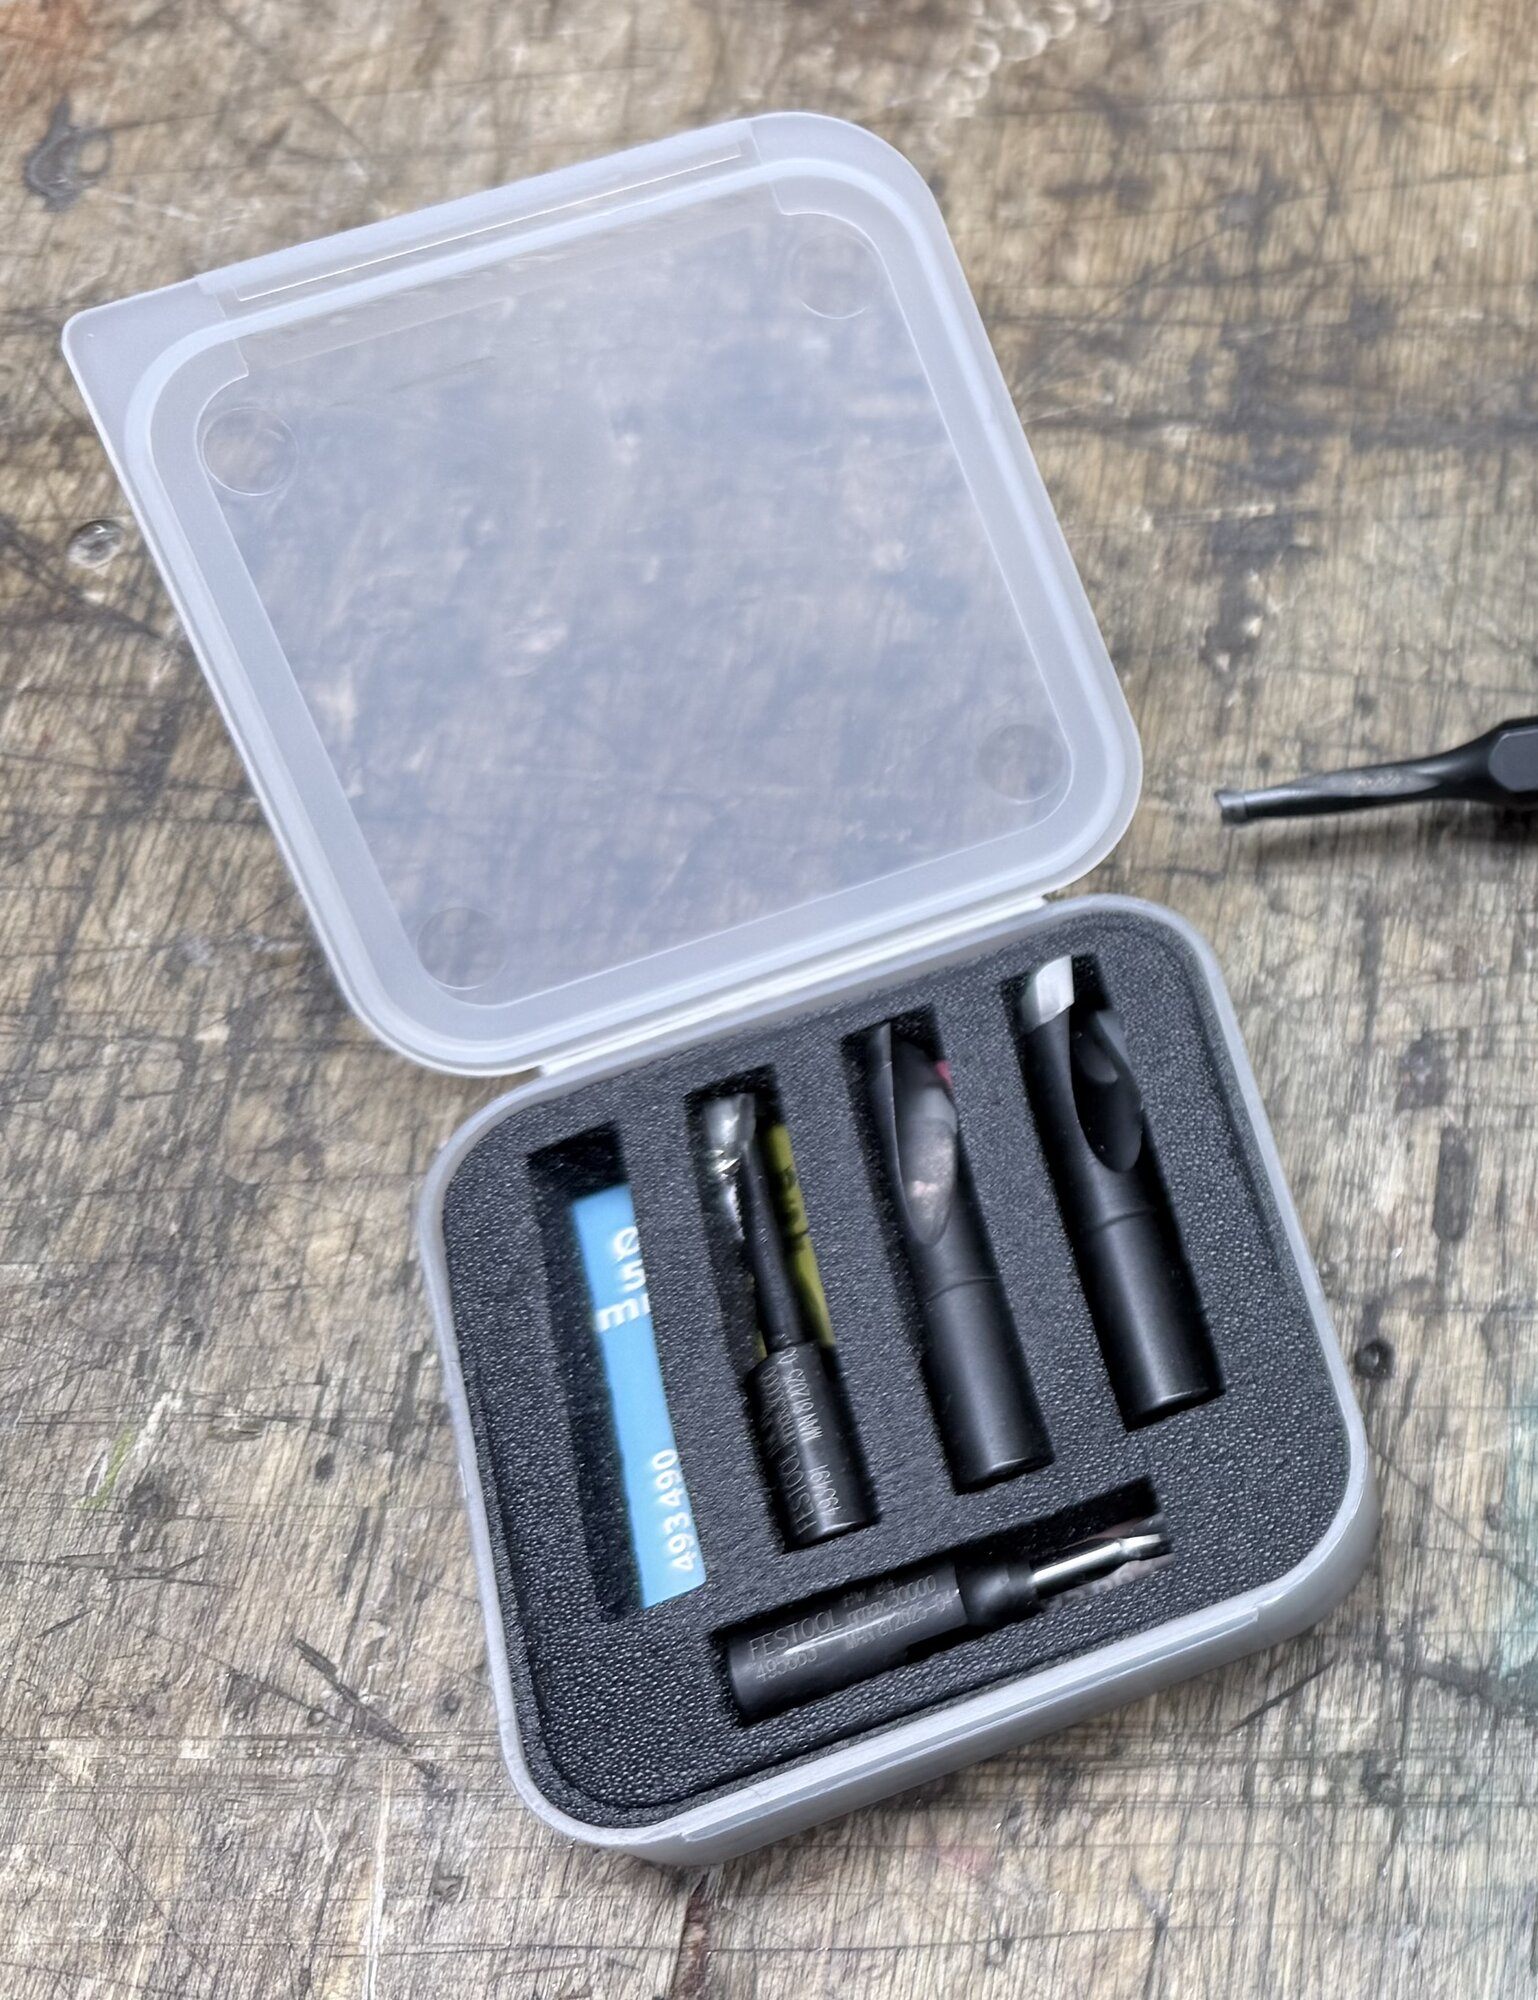
\includegraphics[width=0.3\textwidth]{bilder/domino-fraeser.jpg}\\[1mm]
		{\footnotesize DOMINO-Fräser in der Aufbewahrungsbox.}
	\end{center}

	\subsection{Typische Fehler}
	\begin{itemize}
		\item \textbf{Teile nicht bündig:} Fräsanschlag nicht immer auf derselben Seite aufgelegt oder Höhe zwischendurch verstellt.
		\item \textbf{Teile lassen sich seitlich nicht ausrichten:} alle Langlöcher eng gefräst. Nur das erste eng, die weiteren weit.
		\item \textbf{Fuge bleibt offen:} Frästiefe zu gering oder Späne im Langloch. Langlöcher ausblasen bzw.\ aussaugen, Frästiefe prüfen.
		\item \textbf{Langloch verlaufen oder ausgefranst:} Fräse beim Eintauchen nicht fest angedrückt, zu schnell eingetaucht oder Fräser stumpf.
		\item \textbf{Absaugung schwach:} Absauganschluss oder Schlauch verstopft, Sauger voll.
	\end{itemize}

	\subsection{Pflege und Prüfung}
	\begin{itemize}
		\item Fräse und Motorlüftung regelmäßig von Staub reinigen.
		\item Kabel, Fräser und Anschläge regelmäßig prüfen. Stumpfe oder beschädigte Fräser aussortieren.
		\item Elektrische Prüfung nach DGUV Vorschrift 3 gemäß Prüffrist.
		\item Wartung nur durch Betreuer mit gezogenem Netzstecker.
	\end{itemize}

	\section{Quellen}
	Die Formulierungen und Zeichnungen dieser Einweisung sind eigenständig erstellt; die Zeichnungen sind mit TikZ gezeichnet und zeigen die Fräse schematisch. Sachliche Angaben (technische Daten, Sicherheitsregeln) beruhen auf den Angaben des Herstellers und allgemein bekannten Regeln. Maßgeblich ist die Originalbetriebsanleitung von Festool, die der Maschine beiliegt (Links siehe oben). Festool hat dieses Dokument weder geprüft noch übernimmt es dafür eine Haftung.

	Die Fotos der Dübelfräse sind im FAU FabLab entstanden und stehen wie das Dokument unter CC BY-SA 3.0. Das Foto des Langlochs stammt von Pete Brown (Flickr, CC BY 2.0, Ausschnitt); Nachweise in \texttt{bilder/QUELLEN.md}.

	\ccLicense{festool-duebelfraese-einweisung}{Einweisung Festool-Dübelfräse DOMINO}

\end{document}
